%Tipo de Documento [Conferencia]

\documentclass[conference]{IEEEtran}

%BIBLIOTECAS

% Este paquete se utiliza para generar texto o graficas de relleno.
%\usepackage{blindtext, graphicx}
%Biblioteca para graficas
\usepackage{graphicx}
%Biblioteca para lectura de caracteres ortográficos (tildes..etc. ) 
\usepackage[utf8]{inputenc}
%Biblioteca para graficos vectrizados.svg 
\usepackage{svg}
%Biblioteca para enumerar figuras tablas.. etc en español 
\usepackage[spanish, es-tabla]{babel}


%INICIO DEL DOCUMENTO
\begin{document}


% TITULO DEL PAPER
\title{Hacia la Web Semántica Legíslativa del Congreso de la República de Colombia}


% NOMBRE DE LOS AUTORES
\author{Jesús Pinzón Ortiz\\
	Estudiante Maestría en Ciencias de la Información y las Comunicaciones\\
código Estudiantil 20151295007\\
Universidad Distrital 'Francisco José de Caldas'\\
Email: jpinzono@gmail.com\\ \\
Asígnatura: Tendencias de la Ingeniería de Software}


\maketitle

%Iniciar Abstract
\begin{abstract}
	Este trabajo de investigación, realiza un estudio de todo lo concerniente a plantear las posibles soluciones de implementar la Web Semántica Legíslativa para el Congreso de la República de Colombia. \\ \\
	Se hace una descripción de la situación actual en lo relacionado a la Informática Legíslativa y se hace un planteamiento de la implementación de la Web Semántica Legíslativa; basados en las buenas prácticas y lecciones aprendidas, que ya algunos pocos parlamentos del mundo ya la han adoptado en la gestión eficiente de información legislativa, en pro de tener a disposición del público en general, la transparencia de la información y la disposición libre de ser utilizada en cualquier ambiente ya sea de consulta investigativa o para generar más conocimiento de la informática legíslativa.  Y aquellos Congresos que no la tienen, pueden contar con un avance actualizado y maduro de esta técnologia que les proporciona un proceso más rápido en su futura implementación, incluso haciendo convenios internacionales de mutua colaboración; para así, poder brindar una mejor información Legíslativa y transparencia a la ciudadanía en general del quehacer legislativo del Congreso de Colombia. \\ \\
	Dado que nuestro Congreso colombiano, no poseé ni tan siquiera la puesta en marcha de los datos abiertos, la finalidad de este trabajo investigativo es dejar definido un plan de implementación de los datos abiertos legíslativo (XML legislativo), que es como el punto de partida de toda iniciativa hacia la Web Semántica; y dejar definido las herramientas necesarias para definir la Web Semántica Legíslativa para el Congreso de Colombia.
\end{abstract}


%Iniciar Palabras Clave Formato IEEE
\begin{IEEEkeywords}
Informática Legíslativa, Datos Abiertos Legislativos, XML Legíslativo, Web Semántica Legíslativa, RDF/XML, OWL.
\end{IEEEkeywords}


%SECCIÓN 1. INTRODUCCIÓN 
\section{Introducción}
	En la tendencia de Ingeniería de Software y del mundo tecnológico se ha venido acuñando el termino 'Legislativo' para referirse a todo lo relacionado en el ámbito del tratamiento de la información producida y procesada por los Parlamentos y/o Congresos. No se conoce a quién se de la autoría de estos términos referentes al quehacer legislativo, como son: Informática Legislativa, XML Legislativo y Web Semántica Legislativa, Ontología Legislativa, entre otros.\\\\
	El congreso de Colombia, cuenta con dos sitos web (www.senado.gov.co y www.camara.gov.co) para informar a la ciudadanía en general de los debates de proyectos, actos legislativos, control politico y otros servicios; pero la tecnología es la web 2.0 (repositorio de archivos legislativos con accesos hipervinculados). \\ \\
	Lo que se pretende con este trabajo, es sentar los lineamientos necesarios para avanzar y actualizar hacia la demoninada web 3.o Web Semántica, pero ya en el ámbito Legislativo 'Web Semántica Legislativa', que es ponerle ya significado o conocimiento a estos repositorios de información pero de una manera estructurada (XML Legislativo) y con significado ('Ontologia Legislativa'). \\ \\ 
	Como el punto de partida de esta iniciativa es lograr el XML Legislativo, se dará un planeamiento presupuestado para su implementación en el Congreso de Colombia.

%PARA INSERTAR FIGURAS, IMAGENES 
%		\begin{figure}[h]
%			\centering
%			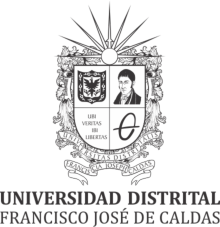
\includegraphics[width=0.2\textwidth]{escudoudblancoynegro}
%			\caption{Escudo Universidad Distrital Francisco Jóse de Caldas}
%		\end{figure}
%SECCIÓN 2.  
\section{Metodología}
Se tiene previsto la siguiente metodología:
\begin{itemize}
   \item[$1.$]	Estudiar y Realizar una investigación sobre la capacidad instalada de Informática Legislativa en la Cámara de Representantes tanto de software como de hardware y de repositorio de datos legislativos para poder dimensionar la solución en informática legislativa y particularmente para proponer  la implementación de la Web Semántica Legislativa para el Congreso de Colombia.\\
   \item[$2.$]	Estudiar y Realizar una búsqueda del estado del arte y de las buenas prácticas a nivel de parlamentos europeos y en particular los parlamentos del continente americano (por ej. Chile, Brasil, etc); cuyas practicas hayan sido exitosas; con el fin, de ver su potencial de implementación en nuestro Parlamento Colombiano. \\
   \item[$3.$]	Proponer un plan metodológico de implementación de la Web Semántica Legislativa para la Cámara de Representantes, estableciendo todos los recursos necesarios para llevarlo a cabo.\\
   \item[$4.$] Proponer un plan de implementación del XML Legislativo para el Congreso de Colombia. Con base a la data set del total de los leyes sancionados por la Presidencia de Colombia, desde los años 1986 a 2015.
\end{itemize}
 
%SECCIÓN 3.  
\section{Sistema de Información actual (Definción de la problemática)}
	Como este trabajo investigativo tendrá apertura a convenios con parlamentos que tiene soluciones exitosas en Web Semántica Legislativa, se hace necesario, en primer instancia hacer una descripción del entorno y organización del Congreso de Colombia.
    En seguida se hará una descripción del Sistema de Información actual, como se opera el repositorio de Información Legislativa
	
%SUBSECCIÓN 3.A  TITULO SUBSECCIÓN
\subsection{Congreso de la República de Colombia}
    En primera instancia, ubiquemos dentro del organigrama del estado de la República de Colombia, el Congreso que conforma la Rama Legíslativa
 %PARA INSERTAR FIGURAS, IMAGENES 
    \begin{figure}[h]
 	  \centering
 	  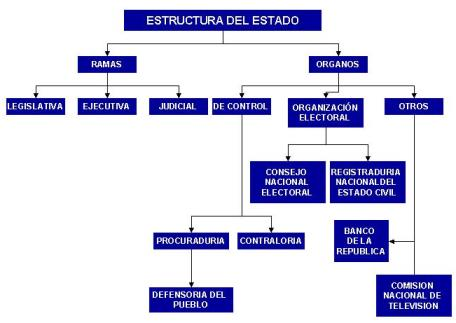
\includegraphics[width=0.5\textwidth]{EEC2}
 	  \caption{Estructura del estado de la República de Colombia}
    \end{figure}   
    Y como Rama Legíslativa, el Congreso de Colombia es bicameral, o sea, lo conforma una cámara alta 'SENADO' y una cámara baja 'CAMARA DE REPRESENTANTES'. Cada una de ellas, tiene Dependencias administrativas (Dirección Administrativa, Financiera, Jurídica, Sistemas, etc.) y Dependencias Legislativas (Mesa Directiva, Secretaria General y Comisiones); regidas por el Reglamento del Congreso de Colombia (Ley 5 de 1992).
    \begin{figure}[h]
    	\centering
    	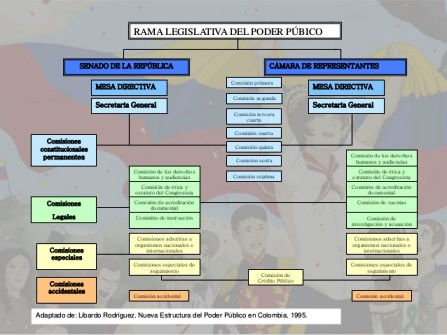
\includegraphics[width=0.5\textwidth]{RLorga}
    	\caption{Organigrama de la Rama Legislativa de Colombia (Congreso de Colombia)}
    \end{figure} 
    Dentro de las funciones que cumple el Congreso de Colombia, como Rama Legistlativa del estado, su principal Función es la legislativa: Para elaborar, interpretar, reformar y derogar las leyes y los códigos de nuestra Constitución.
    \begin{figure}[h]
    	\centering
    	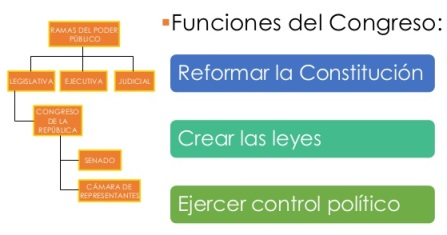
\includegraphics[width=0.5\textwidth]{RLfuncion}
    	\caption{Funciones del Congreso de Colombia}
    \end{figure}
    
 %SUBSECCIÓN 3.B  TITULO SUBSECCIÓN
 \subsection{Repositorio Legislativo del Congreso de Colombia}
    Existen varios portales web que son repositorios de las leyes de Colombia, entre ellos estan el de la Presidencia de la República de Colombia www.presidencia.gov.co, el SENADO de Colombia www.secretariasenado.gov.co y la CAMARA DE REPRESENTANTES www.camara.gov.co; existen otras entidades del gobierno que fijan las leyes que le consiernen o que regulan su interactuar con el estado y demás entidades. Ya el repositorio físico de las leyes, se encuentra un el ARCHIVO LEGISLATIVO del Congreso de Colombia (dependencia adscrita a la Secretaria General). \\ \\    
    Específicamente para el Congreso de Colombia se cuenta con los portales web del SENADO www.senado.gov.co, www.secretariasenado.gov.co, www.comisionseptimasenado.gov.co y de la CAMARA DE REPRESENANTES www.camara.gov.co.  En donde podras consultar, además de las leyes, los proyectos de ley, actos legislativos, ordenes del dia y varios temas del quehacer legislativo del Congreso de Colombia.
    \begin{figure}[h]
    	\centering
    	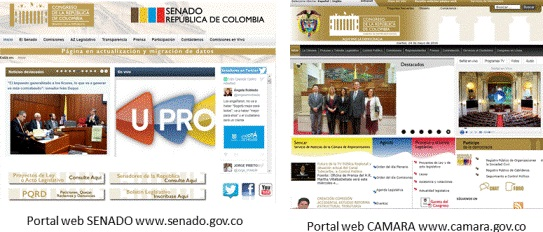
\includegraphics[width=0.4\textwidth]{portales-congreso}
    	\caption{Portales web del Congreso de Colombia}
    \end{figure}
    
 %SUBSECCIÓN 3.C  TITULO SUBSECCIÓN
 \subsection{Marco normativo de las TIC en Colombia}    
    En Colombia, el uso de las Tecnologías de la Información y las Comunicaciones, tomo fuerza desde la década de los noventa, en el marco de los distintos procesos de modernización del Estado; normatividad orientada a reducir la brecha digital y a promover la eficiencia y transparencia del Estado. \\ \\
    La directiva presidencial 02 de 2000, creó la Agenda de conectividad, y el documentos CONPES 3072 de 200, marcan el inicio de políticas orientadas a impulsar la implementación de la Estrategia de Gobierno Electrónico en Colombia. Y en 2008, con la expedición del Decreto 1151 se establece los lineamientos generales de la Estrategia de Gobierno en Línea de Colombia, y hace la obligatoriedad de que las entidades públicas deben implementar los lineamientos que en esta materia expida el MINTIC (Ministerio de las TIC).\\ \\ 
    La ley 1341 de 2009, "Por la cual se definen principios y conceptos sobre la sociedad de la información y la organización de las Tecnologías de la Información y las Comunicaciones TIC.."; entre otros, establece que las TIC deben servir al interés general y es deber del Estado promover su acceso eficiente y en igualdad de oportunidades a todos los habitantes del territorio nacional.  Y en el año 2011 se expidió la ley 1437, por medio de la cual se expide el código de procedimiento administrativo y de lo cotencioso administrativo; en materia de TIC, esta ley incorpora en el procedimiento administrativo los medios electrónicos, como la solicitud y prestación de servicios por medios electrónicos. \\ \\
    En caso específico para el Congreso de Colombia, en el año 2007 con la expedición de la ley 1147, se crea la Comisión Especial de Modernización y sus Unidades Coordinadoras de Asistencia Técnica Legislativa y Atención Ciudadana del Congreso de Colombia. Siendo, entre otros temas, la encargada de estudiar, proponer y crear los procesos de modernización dentro del Congreso, a través del Sistema de Información Parlamentaria y otros medios. \\ \\
    
    
  %SUBSECCIÓN 3.D  TITULO SUBSECCIÓN
  \subsection{Datos Abiertos de Colombia} 
    El portal web de los Datos Abiertos de Colombia www.datos.gov.co, se encuentra de manera unificada, todos los datos publicados por las entidades públicas de Colombia en formato abierto, con el fin de que sean usados por cualquier persona para desarrollar aplicaciones o servicios de valor agregado, hacer análisis e investigación, ejercer labores de control o para cualquier tipo de actividad comercial o no comercial.      \\ \\  
    A mediados de 2010, Berners-Lee estableció una clasificación de cinco categorías para puntuar la calidad de los datos abiertos2. Esta categorización se ha convertido en un principio técnico a partir del cual diseñar una primera ruta de trabajo en la construcción progresiva de plataformas de datos abiertos.
    \begin{figure}[h]
    	\centering
    	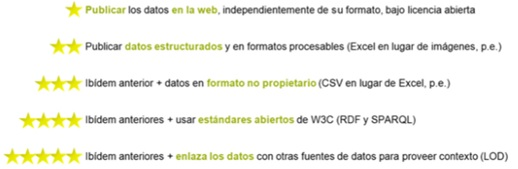
\includegraphics[width=0.5\textwidth]{datos-abiertos-col}
    	\caption{Modelo de las 5 Estrellas \\ \small Fuente: http://inkdroid.org/jo5urnal/2010/06/04/the-5-stars-of-open-linked-data/}
    \end{figure}
    Datos Abiertos y la Estrategia de Gobierno en línea. La apertura de datos busca un mayor acceso a la información pública para diversos propósitos comerciales y no comerciales que facilitan la transparencia, la participación y la colaboración. Igualmente, busca la generación de servicios de valor agregado a la sociedad en general, a través del desarrollo de aplicaciones y servicios realizados por las  comunidades de desarrollo, la industria de tecnologías de información, la academia o cualquier ciudadano.
    \begin{figure}[h]
    	\centering
    	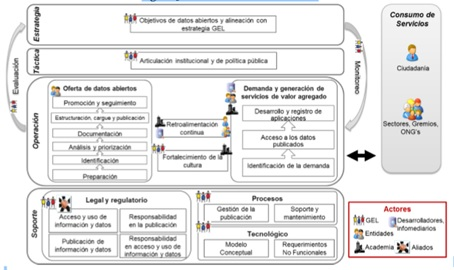
\includegraphics[width=0.5\textwidth]{modelo-datos-col}
    	\caption{Modelo de Datos Abiertos en Colombia}
    \end{figure}
    Haciendo una búsqueda en el portal de datos abiertos de Colombia www.datos.gov.co, no se encuentra datos relacionados con la productividad del Congreso de Colombia (a fecha mayo de 2016) o sea bajo entidades como SENADO y CAMARA DE REPRESENTANTES, no se encuentra archivos de datos legislativos.  

 %SUBSECCIÓN 3.E  TITULO SUBSECCIÓN
 \subsection{Inventario de Información Legislativa del Congreso de Colombia}   
	
	Como ya se indico en un númeral anterior, el repositorio físico de las leyes, se encuentra en el dependencia ARCHIVO LEGISLATIVO del Congreso de Colombia; pero el repositorio digital, esta consignado principalmente en los sitios web de SENADO www.senado.gov.co, www.secretariasenado.gov.co y CAMARA DE REPRESENTANTES www.camara.gov.co; y quien las ejecuta y sanciona, la PRESIDENCIA de Colombia www.presidencia.gov.co.  \\ \\
	Estos contenidos de la producción legíslativa del Congreso de Colombia, se encuentran, la gran mayoría (aprox. 80 porciento), en la web, bajo HTML (textos hipervinculados a fuentes primarias de información); aunque algunos están en formato pdf y otros en word.\\ \\
	A continuación relaciono la cantidad de leyes por años que fueron sanciondas por la Presidencia de Colombia y su fuente de consulta a sus correpondientes textos esta en los portales (en HTML): de las leyes de los años 1968 a 1991 esta en www.camara.gov.co (ftp://ftp.camara.gov.co/camara/basedoc/arbol/1889.html y ftp://ftp.camara.gov.co/camara/basedoc/arbol/1006.html) y las leyes de los años 1992 hasta la fecha, se encuentran en www.secretariasenado.gov.co (http://www.secretariasenado.gov.co/senado/basedoc/arbol/1120.html). \\
		%Iniciar Tabulación 
		% c=centrado 
		% | = Línea de division de la tabla
			\begin{table}[h]
				\centering		
				\begin{tabular}{|c|c|c|r|c|c|c|}
					
					\multicolumn{ 3}{|c|}{{\bf Cantidad de Leyes (1968 a 1991)}} &            & \multicolumn{ 3}{|c|}{{\bf Cantidad de Leyes (1992 a 2015)}} \\
					
					{\bf AÑO} & {\bf RANGO} & {\bf TOTAL} &            &  {\bf AÑO} & {\bf RANGO} & {\bf CANTIDAD} \\
					
					1968 &    1 a 105 &        105 &            &       1992 &     1 A 33 &         33 \\
					
					1969 &     1 a 41 &         41 &            &       1993 &   34 A 106 &         73 \\
					
					1970 &     1 a 24 &         24 &            &       1994 &  107 A 179 &         73 \\
					
					1971 &     1 a 47 &         47 &            &       1995 &  180 A 252 &         73 \\
					
					1972 &     1 a 21 &         21 &            &       1996 &  253 A 345 &         93 \\
					
					1973 &     1 a 71 &         71 &            &       1997 &  346 A 419 &         74 \\
					
					1974 &     1 a 28 &         28 &            &       1998 &  420 A 490 &         71 \\
					
					1975 &     1 a 57 &         57 &            &       1999 &  491 A 552 &         62 \\
					
					1976 &     1 a 61 &         61 &            &       2000 &  553 A 635 &         83 \\
					
					1977 &     1 a 56 &         56 &            &       2001 &  636 A 730 &         95 \\
					
					1978 &     1 a 64 &         64 &            &       2002 &  731 A 793 &         63 \\
					
					1979 &     1 a 74 &         74 &            &       2003 &  794 A 872 &         79 \\
					
					1980 &    1 al 47 &         47 &            &       2004 &  873 A 939 &         67 \\
					
					1981 &    1 al 85 &         85 &            &       2005 & 940 A 1004 &         65 \\
					
					1982 &    1 al 66 &         66 &            &       2006 & 1005 A 1121 &        117 \\
					
					1983 &    1 al 30 &         30 &            &       2007 & 1122 A 1181 &         60 \\
					
					1984 &    1 al 55 &         55 &            &       2008 & 1182 A 1269 &         88 \\
					
					1985 &   1 al 137 &        137 &            &       2009 & 1270 A 1371 &        102 \\
					
					1986 &    1 al 81 &         81 &            &       2010 &  1372 A 1430 &         59 \\
					
					1987 &    1 al 61 &         61 &            &       2011 & 1431 A 1504 &         74 \\
					
					1988 &    1 al 89 &         89 &            &       2012 & 1505 A 1607 &        103 \\
					
					1989 &    1 al 92 &         92 &            &       2013 & 1608 A 1702 &         95 \\
					
					1990 &    1 al 61 &         61 &            &       2014 & 1703 A 1748 &         46 \\
					
					1991 &    1 al 23 &         23 &            &       2015 & 1749 A 1771 &         23 \\
					
				\end{tabular}  
				\caption{Inventario de leyes por año en Colombia}
				\label{inventario_leyes}
			\end{table}
	
	La Información recopilada y que esta en los repositorios ya mencionados anteriormente, se escogió las leyes de Colombia ya sancionadas y aplicadas en Colombia, desde el año 1968 a 2015, porque se encuentran bajo un mismo esquema estructural en formato HTML; las demás se encuentran en impreso en el 'Archivo Legislativo' y algunas están escaneadas y están en formato PDF.  
    
			
	%Para Citar la bibliografia Utilizada
	%\cite{biblio2}
	
		%Iniciar Tabulación 
		% c=centrado 
		% | = Línea de division de la tabla
	%	\begin{table}[h]
	%		\centering		
			
	%		\begin{tabular}{|c|c|c|}
	%			\hline ESTADÍSTICO & SALDO INICIAL & SALDO FINAL \\ 
	%			\hline 1  & 460 & 214 \\ 
	%			\hline 2  & 314 & 213 \\
	%			\hline 3  & 200 & 210 \\
	%			\hline 4  & 500 & 53  \\
	%			\hline 5  & 234 & 76  \\
	%			\hline 
	%		\end{tabular}
	%		\caption{Parámetros Estadísticos }
	%		\label{tabla_parametros}
	%	\end{table}


%SUBSECCIÓN A.  TITULO SUBSECCIÓN
%\subsection{Subsección XX }
%	texto aqui
%Para Citar la bibliografia Utilizada
%\cite{biblio1}
	
	%FORMULAS
	 %Centrar
	 %\begin{center}
	 	% Se llama el ambiente matemático entre signos $
	 %	$E = mc^{2}$
	 %\end{center}

%SECCIÓN 4.  
\section{Objetivos}
   \textbf{Objetivos}: Asesorar y realizar el planteamiento  de la Web Semántica Legislativa para la Cámara de Representantes, que facilite la divulgación de información legislativa en medios masivos de comunicación. Y como objetivos específicos:%\\
   \begin{itemize}
   	  \item Realizar un planteamiento de como sería la web semántica legislativa para el Congreso de Colombia.%\\
   	  \item Elaborar un inventario de Datos Abiertos Legislativos (si los hay) o en su defecto, realizar un plan para el levantamiento de los XML Legislativo, siguiendo una metodología propuesta según una estructura ajustada al quehacer legislativo, para las leyes de la República de Colombia (desde el año 1968 hasta el año 2015), estableciendo un estimativo de tiempo y de presupuesto.%\\
   	  \item Proponer una infraestructura física – tecnológica y organizacional que garanticen la implementación de la Web Semántica Legislativa para el Congreso Colombiano.%\\ 
   \end{itemize}


%SECCIÓN 5.  
\section{De la Web Actual a la Web Semántica}
%Para Citar la bibliografia Utilizada
%\cite{biblio1}
   Me permito hacer una ilustración de lo que ha sido la evolución del Internet WWW, a través de sus diferentes fases (Web 1.0, Web 2.0, Web 3.0 e incluso Web 4.0), junto con las herramientas de software mas significativas
   \begin{figure}[h]
   	\centering
   	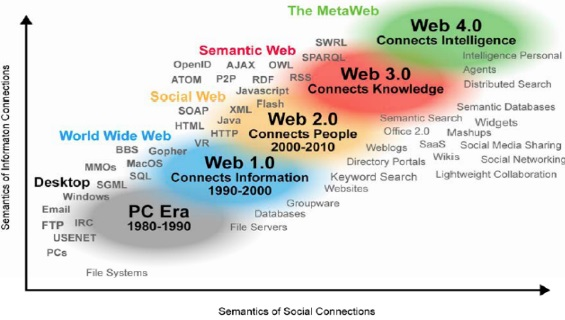
\includegraphics[width=0.5\textwidth]{ws-evolucion-proy}
   	\caption{Proceso evolutivo de la Web}
   \end{figure}
   Otro punto de vista de describir esta evolución de la WWW, es através de las herramientas conceptuales que manejan e interacciones con sus componentes.
   \begin{figure}[h]
   	\centering
   	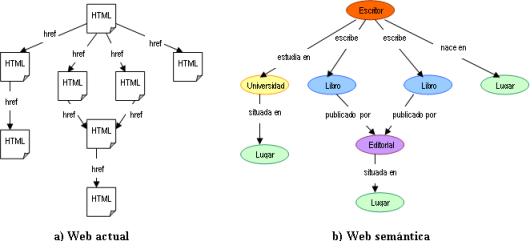
\includegraphics[width=0.5\textwidth]{ws-actual-ws2}
   	\caption{Web Actual vs. Web Semántica}
   \end{figure}
   
   
%SUBSECCIÓN 5A.  TITULO SUBSECCIÓN
\subsection{De la web actual (web 2.0-web social-HTML)}
   La web actual 2.0 o web social, es un medio muy económico para el acceso al conocimiento explicito, servicios, entretenimiento, comercio y negocios electrónicos, etc. Las búsquedas actuales se basan en “palabras clave”; estas escrutan la red a la búsqueda de nuevos documentos, pero no tratan de “entenderlos” sino que se limitan a extraer sus palabras, bien es cierto que de forma muy eficiente. \\ \\
   En la web 2.0, el marcado de datos se realiza mediante HTML, orientado sobre todo a la transmisión de los documentos y su correcta presentación, y queda muy por detrás de las posibilidades ofrecidas por los lenguajes de marcado, diseñados como medio de interconexión entre la gestión de datos y la ofimática documental. \\ \\
   Como es sabido HTML (Hypertex Markup Language) se ha convertido en un lenguaje de inmensa popularidad durante los últimos años. También debemos notar que nos hemos encontrado con sus propias limitaciones, que algunas de ellas se han querido subsanar con scripts, javascripts, Active X, HTML dinámico, etc; pero en la realidad todas estas herramientas no aportan una solución global a las limitaciones del HTML. \\ \\
   HTML, no es un lenguaje de programación, es un lenguaje de especificación de contenidos para un tipo específico de documentos SGML. Es decir, mediante HTML podemos especificar, usando un conjunto de marcas, cómo va a representarse la información en un navegador o browser. La facilidad de uso y la particularidad que no es propiedad de nadie, hizo al HTML el sistema idóneo para compartir información en Internet. La expansión de Internet le ha dado una posición de privilegio y ha hecho que la idea inicial se modifique considerablemente.\\ \\
   Con el HTML se tiene involucrada el uso y aplicabilidad del hipertexto, que permite generar un espacio “virtual” de información —y de experiencia— en la medida en que documentos, medios, emisores y receptores anteriormente dispersos y alejados en el espacio quedan ahora reunidos en un espacio en el que todos se encuentran en concreto a un clic del ratón o de otro dispositivo homólogo. \\ \\
   El marcado de datos que se realiza mediante HTML en la World Wide Web WWW se orienta sobre todo a la transmisión de los documentos y su correcta presentación, y queda muy por detrás de las posibilidades ofrecidas por los lenguajes de marcado, diseñados como medio de interconexión entre la gestión de datos y la ofimática documental. Las limitaciones de la WWW tanto en su implementación del hipertexto como en su capacidad de gestión de datos son precisamente el trampolín del que parte el proyecto de la Web Semántica.
   
 
 %SUBSECCIÓN 5B.  TITULO SUBSECCIÓN
 \subsection{Web Semántica (web 3.0 - XML, RDF, Ontológia}  
    Tim Berners-Lee, el inventor de la Web, se describía una nueva web en la que las aplicaciones eran capaces de entender nuestros deseos, expresados en lenguaje natural, y facilitarnos la información solicitada de forma rápida y eficiente. Desde entonces se han desarrollado varios estándares internacionales, auténticos pilares tecnológicos sobre los que se asentará la web del futuro.\\ \\
    Desde el punto de vista tecnológico cabe precisar algunas de las principales características que aporta la Web Semántica: fundamentalmente, la anotación del contenido mediante lenguajes de marcado (XML) (Arellano, Nogales y Martín, 2003), la definición de estándares de descripción de documentos (XML Schema), el establecimiento de interconexiones entre etiquetas y datos etiquetados (RDF), la definición de esquemas de descripción de recursos y de relaciones entre datos (RDF Schema) y la construcción de ontologías legales distribuidas (OWL) para facilitar la navegación, recuperación y explotación de la información legal.
    \begin{figure}[h]
    	\centering
    	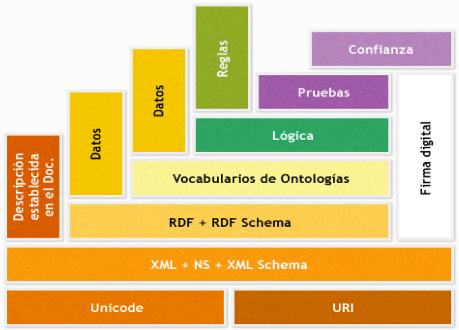
\includegraphics[width=0.5\textwidth]{ws-arquitectura2}
    	\caption{Arquitectura de la Web Semántica}
    \end{figure}
    La web semántica, consiste en una serie de lenguajes distribuidos por capas que permiten la gestión de los objetos del conocimiento y su tratamiento como datos, a partir de lenguajes de anotación semántica, como: RDF (Resource Description Framework), permite describir mediante tripletas que manifiestan conocimiento factual y terminologico; y OWL (Ontology Web Language), razonar (dentro de ciertos límites) mediante clases y propiedades que modelan formalmente conceptos y las relaciones que hay entre ellos. Son lenguajes de grafos sobre XML (eXtended Mark-up Language).  El resultado es la gestión de la información: el vínculo de hipertextos, la conexión de objetos, y la recuperación de información de la red no a partir de palabras clave, sino a partir de conceptos, es decir, del lenguaje natural mediante el que los usuarios de internet o delas grandes bases de datos se expresan normalmente. \\ \\
    Las segunda generación de Web semántica (o otra dirección), enlaza con la denominada Web de Datos, relacionados con los Servicios Web basados en datos vinculados en abierto o  Datos Enlazados (Linked Open Data, LOD), menos enfocada a ontologías y más centrada en la vinculación de los datos encapsulados, tratados como grandes bases de datos en abierto.  El término ‘datos vinculados’ (Linked Data 2007) se utiliza para escribir el espacio evolutivo de RDF; se refiere a un conjunto de buenas prácticas para publicar y conectar datos estructurados en la red. Estas buenas prácticas han sido adoptadas por un creciente numero de proveedores de datos en los últimos años, que ha llevado a la creación de un espacio global de datos que contiene miles de millones ‘la Web de Datos’ (red de cosas en el mundo, descritas mediante datos en la red); asociado con el concepto del modelo de la nube ‘cloud computing’ (computación en la nube).
    \begin{figure}[h]
    	\centering
    	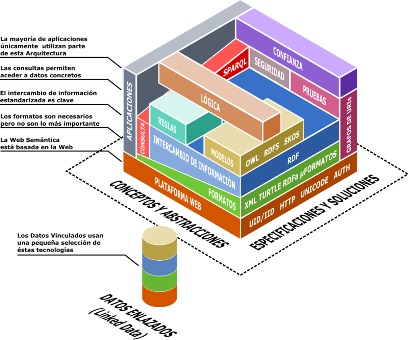
\includegraphics[width=0.5\textwidth]{ws-arquitectura1}
    	\caption{Arquitectura Web Semántica - Datos enlazados}
    \end{figure}
    \textbf{Datos abiertos enlazados (linked open data)}. Los sistemas deben ser construidos bajo el concepto de datos abiertos y enlazados, es decir su contenido se encuentra completamente disponible para ser usado, reusado, redistribuido y enlazado por los ciudadanos. Los datos deben estar abiertos y en RDF o formatos similares. Esto significa que el usuario puede enlazar datos provenientes de diversas fuentes, instituciones u organizaciones, explorar y combinar estos datos de manera libre y sin restricciones de formato y/o copyright para descarga y nuevos desarrollos. Como resultado, los usuarios podrán acceder no sólo a los documentos, sino también información relacionada que describe el contenido, su significado y la relación de los datos. 
    
        
%SECCIÓN 6.  WEB SEMANTICA LEGISLATIVA
\section{Sistema de Información propuesto (Web Semántica Legislativa)}
   Según lo expuesto en la sección 4 "Sistema de Información actual (Definición de la problemática)", y en pro de hacer más eficiente el manejo de la información legislativa y cumpliendo con los lineamientos dados por el grupo Gel 'Gobierno En Línea' de la Presidencia de Colombia,  me permito plantear una solución óptima para tratamiento, almacenaje, la búsqueda y consulta de información legislativa, basados en las mejores prácticas y lecciones aprendidas, que unos pocos Parlamentos del mundo han acogido para este fín, y que se ha convertido en la panacea evolutiva de la web 3.0 'Web Semántica', pero ya aplicada dentro de una estructura bien definida con cuenta la Documentación Legislativa, se conoce con el término de 'Web Semántica Legislativa', conducente a ser adoptada por el Congreso de Colombia. \\ \\ 
   Para el Congreso de Colombia, se debe partir desde su fase mas temprana, o sea, que al solo contar, en el caso especifico de las leyes de Colombia desde 1968 a 2015 en formato HTML, se debe empezar por la conversión de dichos archivos a XML LEGISLATIVO.\\ \\
   La Web Semántica legislativa no sería otra cosa que la aplicación de las posibilidades de la Web Semántica a las características específicas de la información legislativa, y, de manera muy especial, a las necesidades que subyacen tras ellas. Sin embargo, no hay que descartar que los desarrollos con tecnologías semánticas en el campo de la información legislativa no puedan aportar perspectivas nuevas al propio proyecto de la Web Semántica.\\ \\
   Se puede definir la Web Semántica legislativa como un sistema de información, comunicación y documentación de carácter abierto, distribuido e interoperable en la Internet, dotado de las características avanzadas que proporciona la Web Semántica, que evoluciona y se desarrolla con objeto de resolver de forma integrada y sinérgica las necesidades del ciclo completo de la actividad legislativa y de todos sus agentes. A partir de una definición como esta conviene precisar tanto los aspectos tecnológicos como los propiamente legislativos.
   
 %SUBSECCIÓN 6A.  TITULO SUBSECCIÓN
 \subsection{XML LEGISLATIVO o LEGAL XML}  
   XML (Extensible Markup Language) es el lenguaje de marcación estándar promovido por el W3C y adoptado ampliamente a nivel mundial para representar datos y documentos y almacenarlos en forma legible. El concepto principal del lenguaje XML es el de envolver el texto con elementos de anotación, llamados etiquetas o tag, que califican el texto. \\ \\
   Teniendo en cuenta, como se ha señalado, el carácter muchas veces oficial que los documentos parlamentarios representan y que constituyen la expresión de la cultura jurídica de una nación y la elaboración intelectual de un pensamiento político, no todos los estándares XML son adecuados para representar los documentos parlamentarios pues su fragmentación y calificación puede hacer perder la integridad del documento original. De este modo ha surgido el estándar XML Legislativo, denominado Legal XML, que está orientado a conservar íntegro el valor del documento legal y a explotar toda la potencialidad de XML para mejorar el proceso legislativo. \\ \\
   Según el Reporte del Word E-Parliament de 2012 hay un número importante de ventajas en el uso del XML Legislativo, entre las que destacan: favorece el intercambio de documentos entre los propios órganos legislativos y con entidades externas; permite una búsqueda extensas con resultados más precisos; posibilita la vinculación entre documentos e incluso entre secciones del mismo; habilita el acceso a la documentación a través de múltiples canales; homogeniza los formatos de los documentos y en este sentido puede apoyar la técnica legislativa; y garantiza la conservación a largo plazo de los documentos. \\ \\
   Un elemento esencial de este XML legislativo y la técnica aprobada oficialmente por varios países para garantizar la validez jurídica de los documentos legislativos es la firma electrónica, pues asegura: la autenticación del autor, la integridad del documento firmado y el no repudio de la procedencia del mismo. En este sentido, el Instituto Europeo de Normas de Telecomunicaciones (ETSI) y otros organismos de estandarización recomiendan al respecto el uso de XAdES (Firma electrónica avanzada XML), un formato de algoritmos criptográficos de sonido, para la gestión de sobres de firma digital avanzados; en Colombia existen entidades como CERTICAMARA. 
   
 
%SUBSECCIÓN 6B.  TITULO SUBSECCIÓN
\subsection{AKOMA NTOSO}  
   Akoma Ntoso ( "corazones conectados" en el idioma Akan de África Occidental) define un conjunto de representaciones electrónicas simples tecnológicamente neutros en formato XML de los documentos parlamentarios, legislativos y judiciales.  Akoma Ntoso se ha desarrollado en el marco de un proyecto del Departamento de Asuntos Económicos y Sociales de Naciones Unidas para apoyar el acceso abierto en los parlamentos africanos y su mantenimiento es actualmente apoyado por el Plan de Acción de Naciones Unidas Africa i-Parliaments. \\ \\
   \textbf{PRESENTACION, ESTRUCTURA Y SEMANTICA}. Hay cuatro aspectos relevantes para cualquier documento, y en particular para los documentos parlamentarios, legislativos y judiciales:
 \begin{itemize}   
   \item[$1.$]	Contenido - el conjunto real de las palabras y puntuacion que forman las frases del texto;
   \item[$2.$]	Presentación - cómo la información se ve, por ejemplo, el color del texto utilizado en el documento, la fuente utilizada en las partidas y de otras cuestiones de formato;
   \item[$3.$]	Estructura - cómo se organiza la información, por ejemplo, la identificación de algunas partes del texto como títulos, algunas partes como las cláusulas, etc .;
   \item[$4.$]	Semántica - lo que representa la información o medios
 \end{itemize}   
   Los esquemas XML de Akoma Ntoso hacen explícita la estructura y los componentes semánticos de los documentos digitales con el fin de apoyar la creación de servicios de información de alto valor que entregan el poder de las TIC y aumentan la eficiencia y la rendición de cuentas en contextos parlamentario, legislativo y judicial.\\ \\
   El esquema Akoma Ntoso XML hace que los componentes estructurales y semánticos de los documentos legislativos digitales sean totalmente accesibles a procesos informáticos, de ese modo se apoya la creación de servicios de información parlamentaria. \\ \\
   Akoma Ntoso define un modelo de acceso abierto centrado en las siguientes cuestiones:
 \begin{itemize}  
   \item[$1.$]	generación de documentos: debe ser posible utilizar las mismas herramientas para la creación de los documentos, independientemente de su tipo, país, idioma, y el proceso de generación.
   \item[$2.$]	presentación de documentos: debe ser posible utilizar las mismas herramientas para mostrar en pantalla e imprimir en papel de todos los documentos, independientemente de su tipo, país, idioma y el proceso de generación.
   \item[$3.$]	accesibilidad de los documentos: debe ser posible referenciar y acceder a documentos de todo tipos, idiomas, países, etc., convirtiendo la red de referencias explícitas entre los textos en una red de enlaces de hipertexto que permiten al lector a navegar fácilmente y de inmediato a través de ellos.
   \item[$4.$]	Descripción de los documentos: debe ser posible describir todos los documentos, independientemente de sus tipos, idiomas, países, etc., a fin de hacer posible la creación de repositorios, motores de búsqueda, herramientas de análisis, herramientas de comparación, etc.\\
 \end{itemize}    
   Al mismo tiempo, el modelo Akoma Ntoso considera las diferencias que existen en los tipos de documentos individuales, que se derivan del uso de diferentes lenguajes humanos, y que están implícitos en la cultura legislativa de cada país. Por tanto, el modelo de acceso abierto común está diseñado para ser flexible, para apoyar excepciones, y para permitir extensiones lo suficiente como para proporcionar apoyo a todas las características individuales que se pueden encontrar en un conjunto de documentos completo que cubra las diferentes culturas y países.\\ \\
   En estos momentos está siendo adoptado o ha sido introducido como mejor práctica en varios países, como por ejemplo el Senado de Brasil, el Parlamento Europeo, para este efecto se realizan acciones con el objetivo de personalizar y adaptar Akoma Ntoso a sus propios sistemas jurídicos y propósitos de transparencia legislativa. 
   
   
%SECCIÓN 7. CONCLUSIÓN 	
\section{Conclusión}
   A medida que ha evolucionado la web, se ha ido tomando las mejores prácticas y lecciones aprendidas y se han incorporado en la gestión de las entidades como medio de subsistencia y permanencia en este continuo perfeccionamiento del conocimiento tecnológico y del conocimientos humano usando a su favor la plataforma del software y hardware que ha venido evolucionando también a la par; gracias al acompañamiento y estandarización sugerida por su creador WWW Tim Berners-Lee y su equipo del grupo w3c, han introducido desde año 2000 la concepción de la Web Semántica (Breners-Lee, Hendler y Lassile, 2001), en un entorno interoperable de computación distribuida y sobre todo en el intercambio de información entre personas a través de páginas web.\\ \\
   La Web Semántica en ámbito legislativo 'Web Semántica Legislativo' debe ser implementada en la práctica, y su posicionamiento estratégico sobre su viabilidad. Son en especial los entes gubernamentales y las grandes empresas que generan y explotan la información legislativa los que poseen el volumen de datos estructurados y semiestructurados, la visión estratégica, el grado suficiente de formalización de sus procedimientos y los recursos disponibles necesarios para llevarla a cabo.\\ \\
   Ya hay un amplio camino recorrido en lo relacionado a la Web Semántica Legislativa, y como mejores prácticas y lecciones aprendidas y sobre todo en un estándar desarrollado para los Parlamentos, es imperiosa la necesidad del Congreso de Colombia que adopte el estándar AKOMA NTOSO; ya implementado éxitosamente por la Biblioteca del Congreso Nacional de Chile y el Congreso de Brasil (aqui en nuestro continente americano) y otros países del continente europeo y su natal africa. Dando empiezo hacia la Web Semántica del Congreso de Colombia; empezando por implementar el hístorico de las leyes, se tomaría las correspondiente a los años de 1968 a 2015, ya que están en una estructura uniforme y en HTML; se debe hacerse la conversión a XML-adhoc para luego quede fácil su paso a XML AKN (estándar AKOMA NTOSO) y de allí queda lista como datos abiertos enlazados. Ya este estado, queda disponible para que cualquier personal o ente público o privado pueda hacer uso de ellas en sus procesos; y luego mediante ontologías Legislativa, poder hacer uso eficiente para el consumo interno o internacional. Se podría reducir esta brecha digital, si se estable un convenio de colaboración con personal Profesional conocer de esta implementación de la Biblioteca del Congreso Nacional de Chile, los cuales ya muestran voluntad de colaboración. Claro esa, que una vez el grupo técnico adquiera la experiencia y asimile esta tecnología, se procederá a incluir todos los documentos legislativos producidos por el Congreso de Colombia.

	
%SECCIÓN DE APENDICES  
%\appendices
%\section{Prueba de la Primera Zonklar Ecuación}
%	texto aqui
		
	%IMAGEN 
	%\begin{figure}[h]
	%	\centering
	%	
\includegraphics[width=0.2\textwidth]{IngenieriaIndustrial}	%\caption{Proyecto Curricular de Ingeniería Industrial}
	%\end{figure}


%SECCIÓN DE RECONOCIMIENTOS
\section*{Reconocimientos}

	Se agradece al profesor Dr. Jose Nelson Pérez, por habernos ilustrado en temas como la programación literaria, para al presetanción de reportes dinámicos en R y Latex. Lo mismo que el haber planteado temas de mucho interés en cuanto a las tendencias de la Ingeniería de Software en varios campos de la técnologia actual. \\ \\
	También es de reconocer el apoyo dado por la Coordinadora de la Unidad de Asistencia Técnica Legislativa y de otros directivos del Congreso que facilitaron la información para posibilitar la realización del presente trabajo.\\  \\
	A la familia por haberme apoyado y haberme sabido comprender en aquellos espacios de tiempo que se dedicaban antes y que fueron ocupados en el desarrollo de los temas del presente trabajo.

%BIBLIOGRAFÍA

%ENTORNO {thebibliography}
%Permite al autor listar las referencias utilizadas y citarlas en algun punto del texto.

	\begin{thebibliography}{1}
		
	\bibitem{biblio1}
		M. Palmirani, XML LEGISLATIVO: Principios e Instrumentos Técnicos. CIRSFID-Universidad de Bolonia, Traducido: German Gómez V, 2012. 
	\bibitem{biblio2}
		A. Castello, WEB SEMANTICA: RDF Y SGBD QUE LO SOPORTAN, Consultor: Oscar Celma, 2006.
	\bibitem{biblio3}
		F. Garcia, Perspectivas sobre el uso de la Web Semántica en el tratamiento de información y documentación legislativa, España: Universidad de Zaragoza, 2009.
	\bibitem{biblio4}
		M. Carrión, Diseño y Desarrollo de un Modelo Computacional para la Representación del Conocimiento en el dominio de la cooperación Judicial en materia penal, Tesís Doctoral, UED: Departamento de Filología, 2012.
	\bibitem{biblio5}
		P. Casanovas, Derecho-Técnologia-Inteligencia Artificial y Web Semántica. Un mundo para todos y para cada uno, UNAM: Biblioteca Juridica, capitulo 23, pp. 825-887, 2008.
	\bibitem{biblio6}
		M. Gómez and J. Pérez, Una introducción a la Web Semántica, QDQDI1DQ: vol 2 num 2, 2006.
	\bibitem{biblio7}
		N. Casellas, Modelling Legal Knowledge throgh Ontologies. OPJK: the Odontology of Professional Judicial Knowledge, tesis doctoral, 2008. 
	\bibitem{biblio8}
		M. Martínez y otros, Estructura, semántica, extracción de información y XML legislativo: experiencias en la U.de Valladolid. XMLeg, 2007. 	
	\bibitem{biblio9}
		J. Belbis, Estudio de caso. Apertura legislativa en el Cono Sur. Documento de trabajo, 2015. 	
	\bibitem{biblio10}
		E. Gimeno, Elaboración de proyectos de ley en forma colaborativa, abierta y en línea. Tesis/U.Buenos Aires, 2015.	
	\bibitem{biblio11}
	    Y. Amoroso y J. Espinoza, Sociocibernética, Informática Jurídica e Infoética. Buenas prácticas y lecciones aprendidas. UNIJURIS/ASIDER, 2015.
	\bibitem{biblio12}
	    Congreso de los Diputados de España, Parlamentos abiertos, tecnologías y redes para la democracia. 2014.    
	 \bibitem{biblio13}
	    P. Reyes, Datos Gubernamentales Abiertos (Open Data Gov) en: construyendo el e-G y la sociedad del conocimiento. Memorias/UNESCO, 2011.
	\bibitem{biblio14}
	    Congreso de Colombia, Reglamento del Congreso (ley 5 de 1992). Leyes/Ley 5 de 1992, 2014. 
	\bibitem{biblio15}
	    Ministerio de Tecnologías de la Información y las Comunicaciones de Colombia, Lineamientos para la implementación de datos abiertos en Colombia.  MINTIC/CINTEL, 2011. 
	\end{thebibliography}

\end{document}